\section{Механический расходомер}

На практике известно довольно много методов определения
расхода, причем простейшими и поэтому наиболее распространенными
из них являются методы с использованием механических элементов, в
которых поток перемещает или вращает твердое тело. Таким образом, это
перемещение или вращение тела оказывается пропорциональным расходу \cite{physfields}.

Преимуществами турбинных расходомеров по сравнению с расходомерами других типов являются:
\begin{itemize}
    \item линейная зависимость их выходного сигнала от скорости потока в установленном для прибора диапазоне (прямое измерение);
    \item простота электрической схемы, а также относительная простота механической части.
\end{itemize}

Недостатки турбинных расходомеров:
\begin{itemize}
    \item наличие движущихся частей и деталей;
    \item низкая износостойкость;
    \item склонность к загрязнению смолистыми отложениями и парафином;
    \item зависимость показаний счета прибора от фазового состояния среды и направления потока.
\end{itemize}

Однако, несмотря на свои недостатки,
турбинные расходомеры остаются одними из
самых распространенных датчиков расхода
жидкости в геофизике  \cite{physfields}. Типовые конструкции
механических измерителей скорости потока
приведены на рис. \ref{fig:scheme_1}.

\begin{figure}[h]

\begin{subfigure}{0.5\textwidth}
\centering
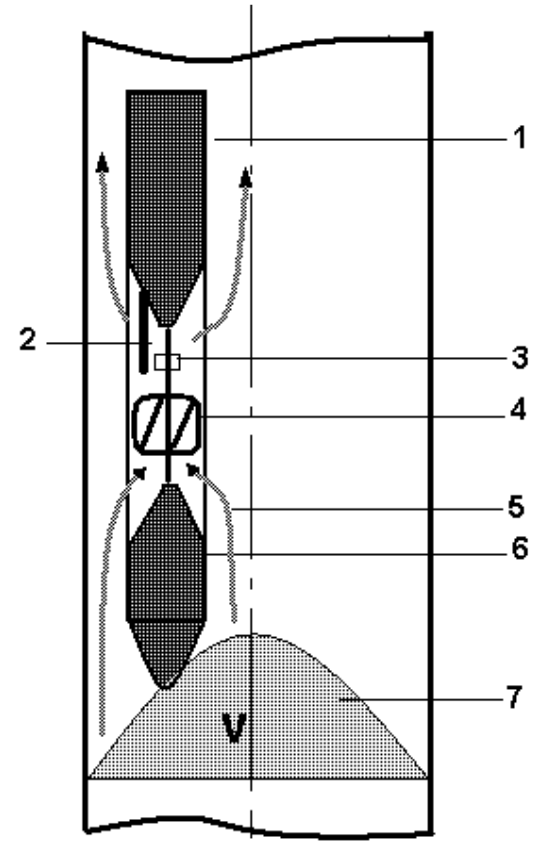
\includegraphics[height=7.5cm]{scheme_1a} 
\caption{Беспакерный расходомер}
\label{fig:subim1}

\end{subfigure}
\begin{subfigure}{0.5\textwidth}
\centering
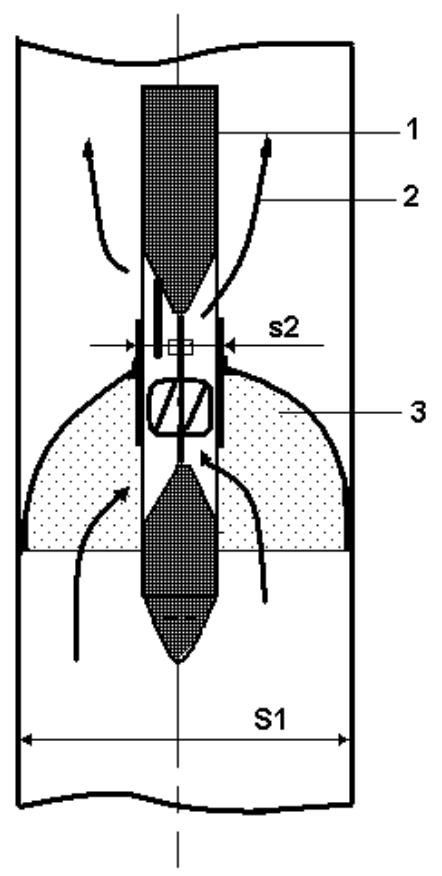
\includegraphics[height=7.5cm]{scheme_1b}
\caption{Пакерный расходомер}
\label{fig:subim2}
\end{subfigure}

\caption{
а)
1~---~корпус прибора; 2~---~датчик вращения турбинки;
3~---~постоянный магнит; 4~---~турбинка;
5~---~линии тока измеряемого потока; 6~---~передний обтекатель;
7~---~эпюра скорости потока в свободной трубе при однофазном потоке
б)
1~---~корпус прибора; 2~---~линии тока исследуемого потока;
3~---~пакерное устройство, перекрывающее скважину;
$S_1$~---~площадь сечение скважины;
$s_2$~---~проходное сечение прибора
}
\label{fig:scheme_1}

\end{figure}

Принцип работы такого расходомера основан на использовании
механической турбины, вращающейся под действием поток
скважинного флюида. При этом, скорость вращения турбины
оказывается пропорциональной расходу \cite{thermodyn}.

\subsection{Пакерный и беспакерный расходомер}

Особенность беспакерного расходомера является его
конструкция, обеспечивающая измерение скорости потока флюида,
свободно обтекающего прибор. При этом корпус прибора может быть
центрирован относительно оси скважины, или смещен к стенке.
Учитывая распределение скорости потока по радиусу скважины,
следует отметить, что измеряемая скорость потока, в общем случае, не
соответствует ни средней, ни максимальной. При пересчете скорости
потока на расход необходимо учитывать реальное сечение канала тока
и искажающее влияние корпуса прибора на структуру потока.
Корректных способов оценки этих взаимовлияний не существует, но
они учитываются в процессе градуировки прибора, выполняемого в
восходящем и нисходящем потоке в трубах различного диаметра \cite{thermodyn}.

Отличительной особенностью пакерного расходомера является
наличие пакерного устройства, управляемого или неуправляемого,
обеспечивающего перекрытие пространства между прибором и стенками
скважины. При этом весь поток жидкости направляется на турбинку
расхо домера, а скорость потока в приборе увеличивается в соответствии с
соотношением:
$${V_2 \over V_1} = {S_1 \over s_2}$$
где $S_1 = \pi R^2$~---~площадь сечения скважины,
$s_2$~---~проходное сечение прибора,
$V_1$~---~средняя скорость потока в скважине,
$V_2$~---~скорость потока в зоне турбинки \cite{thermodyn}.

На рис. \ref{fig:scheme_3}, а изображен дебитомер-расходомер турбинного типа. Измерительным элементом слу­жит разгруженная гидромет­рическая турбинка. Поток жидко­сти, проходя через окна 8 и 11, вращает турбинку 9, на общей оси с которой установлен постоянный П-образный магнит 7. Этот магнит через стенку герметичной каме­ры (из немагнитного материала) управляет установленным в ка­мере магнитным прерывателем тока 6. Принцип действия преры­вателя следующий (рис. \ref{fig:scheme_3}, б). При вращении магнита 7, укреп­ленного на турбинке, магнитная стрелка 12 совершает колеба­тельные движения вокруг оси 16, замыкая и размыкая электричес­кую цепь через подвижный кон­такт 15. Таким образом, в цепи, подключенной к кабелю 1, возни­кают электрические импульсы, число которых, очевидно, совпа­дает с числом оборотов турбинки. Амплитуда колебаний стрелки ограничивается контактом 15 и упором 13. Магнит 14 увеличи­вает время стояния стрелки на контакте. Преимущество магнитного прерывателя — незначитель­ная мощность, требуемая для его работы, а отсюда весьма неболь­шое тормозящее действие на турбинку \cite{mechdebit}.

Пакер 10 рассматриваемого прибора представляет собой чехол из ткани, натянутой между парами пластинчатых пружин. Раскрытие пакера осуществляется электрическим приводом, состоящим из электродвигателя и ходового винта 3. Винт 3, ввинчиваясь в травер­су 4, двигает подвижную трубу 5 относительно корпуса 2 вниз. При этом труба 5, нажимая на пластинки пакера, выгибает их наружу, и, расправляя ткань пакера, перекрывает кольцевое пространство меж­ду дебитомером и колонной. Одновременно с этим окно 8 на трубе 5 совмещается с соответствующим окном в корпусе 2, открывая путь для движения всего потока жидкости через струенаправляющую трубу дебитомера, где установлена турбинка. При обратном направ­лении вращения ходового винта 3 пластинки пакера распрямляются и ткань складывается вокруг прибора.

\begin{figure}[h]
\centering
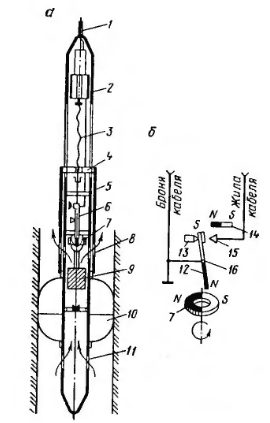
\includegraphics[height=12cm]{scheme_3}
\caption{
Принципиальная схема дебитомер турбинного типа (а) и магнитного прерывателя (б)
}
\label{fig:scheme_3}
\end{figure}

Импульсы тока от прерывателя 6 по кабелю передаются на по­верхность, специальным блоком частотомера преобразуются в по­стоянный ток, который пропорционален числу импульсов и регистрируется регист­ратором геофизической станции. Частота вращения турбины пропор­циональна скорости потока. Коэффициент пропорциональности оп­ределяется градуировкой прибора на специальных стендах или не­посредственно на скважине.

Основной элемент, определяющий
характеристики механического расходомера ---
подшипник оси турбинки (рис. \ref{fig:scheme_2}). В зависимости от качества
его изготовления, зависит как минимальная скорость
измеряемого потока, так и стабильность показаний при
эксплуатации \cite{physfields}.

\begin{figure}[h]
\centering
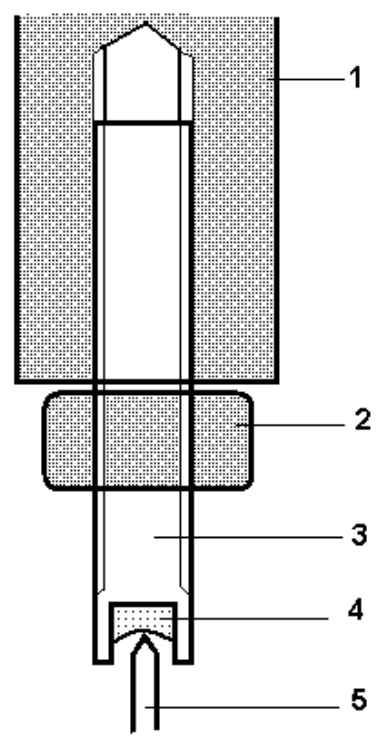
\includegraphics[width=3cm]{scheme_2}
\caption{
Конструктивное исполнение подшипника оси турбинки \\
1~---~корпус прибора, 2~---~контрогайка,
3~---~металлический стержневой корпус подшипника,
4~---~собственно подшипник, корунд или рубин со сферической рабочей поверхностью,
5~---~ось турбинки из высокопрочного металла
}
\label{fig:scheme_2}
\end{figure}

Путем изменения глубины ввертывания корпуса подшипника в
корпус прибора, добиваются минимального вертикального люфта оси
турбинки, которое обеспечивает минимальный тормозной эффект.

Загрязнение подшипника абразивными частицами или
смолистыми отложениями приводит к резкому увеличению сил трения,
которые в свою очередь влияют на передаточную характеристику
датчика. Увеличенный осевой люфт в сочетании с дисбаллансом
турбинки выводит точку контакта оси турбинки с полированной
корундовой поверхности на боковую поверхность, что резко увеличивает
площадь контакта и, соответственно, силу трения в подшипнике.


\subsection{Градуировка и передаточная характеристика}

В процессе градуировки механических скважинных
расходомеров на специальных стендах снимают показания с измерителя,
соответствующие скорости вращения оси турбинки в зависимости от
скорости потока или расхода \cite{thermodyn}. Типовая градуировочная диаграмма
приведена на риc. \ref{fig:graph_1}.

\begin{figure}[h]
\centering
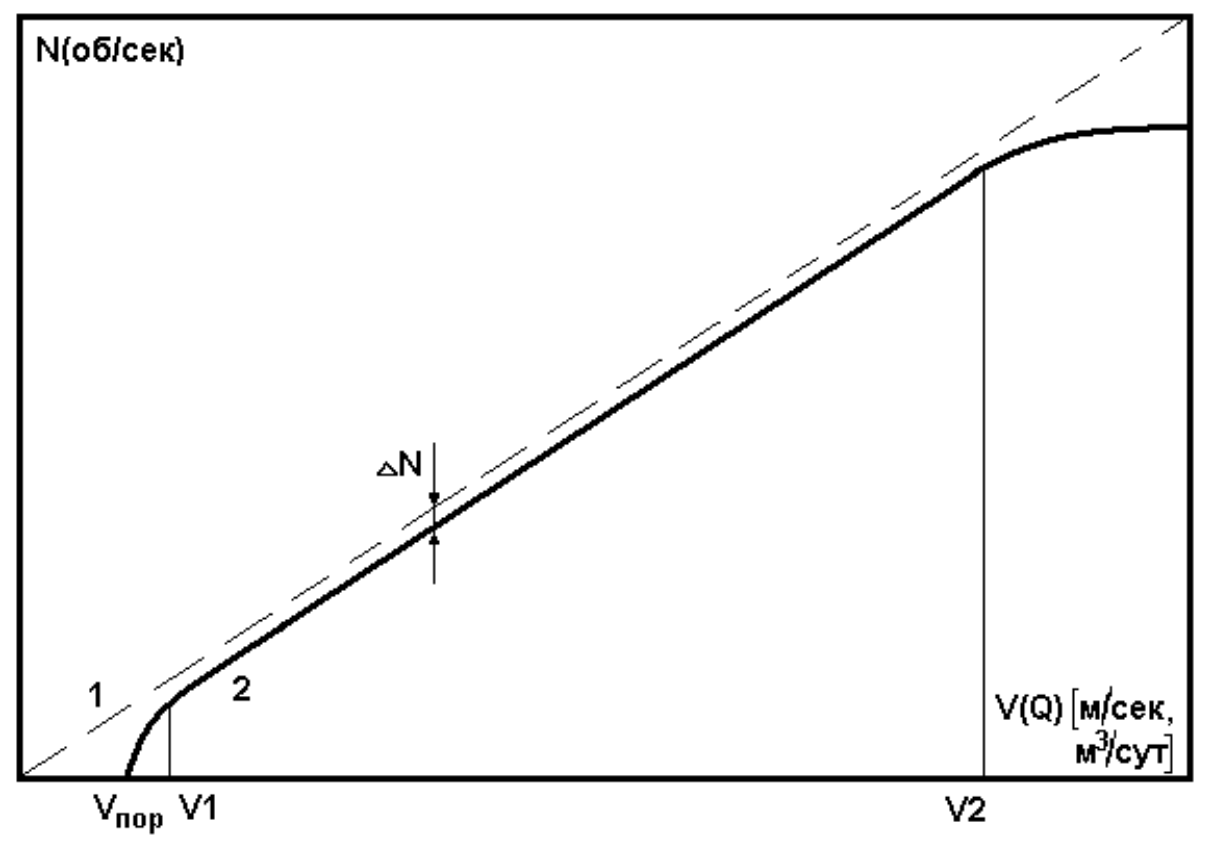
\includegraphics[width=0.5\linewidth]{graph_1}
\caption{
Градуировочная кривая механического расходомера. \\
1~---~передаточная характеристика идеального датчика,
2~---~реальная градуировочная характеристика,
$V_\mathrm{пор}$~---~порог срабатывания датчика (начало вращения),
$V_1 < V_\mathrm{раб} < V_2$~---~диапазон рабочих скоростей датчика
}
\label{fig:graph_1}
\end{figure}

Реальный датчик скорости потока имеет ограничение по скорости
потока как снизу $V_1$, так и сверху $V_2$. Нижний порог $V_1 = V_\mathrm{стр}$ получил
название --- "порог страгивания" и возникает за счет трения в
подшипниках оси турбинки. Кроме того, дополнительный тормозящий
эффект возникает при нарушении статической балансировки турбинки,
особенно заметный в наклонных и горизонтальных скважинах. Верхняя
граница рабочего диапазона $V_2$ определяется началом искажения
линейной зависимости за счет эффекта "проскальзывания" жидкости
мимо турбинки. Если известны значения $V_1$, $V_2$ и диаметр трубы,
легко определить нижний и верхний порог рабочих расходов для
конкретного расходомера из соотношения:
$$Q = VS$$
где $S = \frac 1 4 \pi D^2$~---~площадь внутреннего сечения трубы \cite{thermodyn}.

Пороговые значения скорости потока и диапазон изменения расхода
в эксплуатационной колонне и в НКТ для механических расходомеров,
рассчитанные по данным производителя, приведены в таблицах \ref{table:1} и \ref{table:2}.

\begin{table}[h]
\caption{Пакерный расходомер}
\label{table:1}
%\resizebox{\linewidth}{!}{%
\begin{tabular}{|l|l|l|}
\hline
\multicolumn{3}{|c|}{Диапазон измерения расхода по жидкости}
\\ \hline
\multicolumn{1}{|l}{}
& В колонне $D = 146~\mathrm{мм}$
& В НКТ $D = 73~\mathrm{мм}$
\\ \hline
${Q_1}_\mathrm{min}$
& 0.2~$\mathrm{м^3/час}$ (4.8~$\mathrm{м^3/сут}$)
& 0.05~$\mathrm{м^3/час}$ (1.2~$\mathrm{м^3/сут}$)
\\ \hline
${Q_2}_\mathrm{max}$
& 60~$\mathrm{м^3/час}$ (1440~$\mathrm{м^3/сут}$)
& 15.00~$\mathrm{м^3/час}$ (360~$\mathrm{м^3/сут}$)
\\ \hline 
\end{tabular}%
%}
\end{table}

\begin{table}[h]
\caption{Беспакерный расходомер}
\label{table:2}
\resizebox{\linewidth}{!}{%
\begin{tabular}{|l|l|l|l|l|}
\hline
\multicolumn{2}{|c|}{\multirow{2}{5cm}{\centering Диапазон измерения скорости потока по жидкости}}
& \multicolumn{3}{c|}{Диапазон измерения расхода по жидкости}
\\[12pt] \cline{3-5}
\multicolumn{2}{|c|}{}
& \multicolumn{1}{|l}{}
& В колонне $D = 146~\mathrm{мм}$
& В НКТ $D = 73~\mathrm{мм}$
\\[12pt] \hline
${V_1}_\mathrm{min}$
& 0.006 м/с
& ${Q_1}_\mathrm{min}$
& 0.2~$\mathrm{м^3/час}$ (4.8~$\mathrm{м^3/сут}$)
& 0.05~$\mathrm{м^3/час}$ (1.2~$\mathrm{м^3/сут}$)
\\ \hline
${V_2}_\mathrm{max}$
& 1.755 м/с
& ${Q_2}_\mathrm{max}$
& 60~$\mathrm{м^3/час}$ (1440~$\mathrm{м^3/сут}$)
& 15.00~$\mathrm{м^3/час}$ (360~$\mathrm{м^3/сут}$)
\\ \hline
\end{tabular}%
}
\end{table}

В том случае, когда реальный расход жидкости, или относительная
скорость потока выходят за указанные пределы, механический
расходомер не обеспечивает возможность количественных оценок
измеряемого параметра.

Механические расходомеры должны удовлетворять следующим требованиям:
\begin{itemize}
    \item динамический диапазон (отношение максимального измеряемого дебита к минимальному) для пакерных приборов -- не менее 10, для беспакерных --- не менее 50;
    \item коэффициент нелинейности --- не более $\mathrm{\pm}$3~\%;
    \item нижний предел измерений для пакерных приборов --- не более 5~$\mathrm{м^3 / сут}$, беспакерных --- 20~$\mathrm{м^3 / сут}$;
    \item погрешность измерения скорости вращения турбинки --- не более $\mathrm{\pm}$3~\%;
    \item коэффициент пакеровки прибора при неизменном диаметре колонны --- не менее 0,9;
    \item превышение амплитуды полезного сигнала над уровнем помех --- не менее чем в 5 раз \cite{mechraskhod}.
\end{itemize}

\subsection{Метрологические параметры}

Реальные значения метрологических параметров скважинного
расходомера в условиях эксплуатации могут существенно отличаться
от паспортных значений по следующим причинам:
\begin{itemize}
    \item загрязнение турбинки или подшипников приводит к
          значительному повышению порога страгивания;

    \item механический износ подшипника и искривление оси турбинки
          приводит к возникновению дисбаланса и повышению порога страгивания;
    \item загрязнение, износ, искажение геометрии турбинки существенно
          снижает верхний диапазон регистрируемых скоростей и расходов;

    \item различие плотности или вязкости скважинного флюида
          относительно характеристик технической воды, на которой
          проводится градуировка расходомера, существенно меняет
          метрологические параметры прибора;

    \item отклонение оси прибора от вертикального положения приводит к
          возникновению дополнительного тормозящего момента на оси
          турбинки и искажает его метрологические характеристики;

    \item отклонение оси скважины от вертикали в условиях двух или
          трехфазного потока вызывает существенное искажение профиля
          скоростей по сечению потока и затрудняет возможность
          количественных измерений беспакерныи расходомерами \cite{thermodyn}.
\end{itemize}

Таким образом, метрологические параметры механических
скважинных расходомеров, полученные в идеальных условиях на
специальных стендах, не могут быть рекомендованы для
количественных измерений в скважинных условиях.

\subsection{Измерение}

Для количественных измерений средней скорости потока и оценки
дебита (расхода) флюида рекомендуется метод прямой калибровки
расходомера в скважинных условиях в процессе исследований.
Технология исследований, обеспечивающая учет реальных
метрологических параметров расходомера, построение профиля
притока (поглощения) и количественную оценку расхода флюида,
получила название "расходометрия на скоростях". Для успешной
реализации технологии необходимо проведение серии замеров на
спуске и на подъеме в интервале эксплуатируемых пластов. Для оценки
общего дебита исследования проводятся выше интервала притока в
зоне установившегося потока (рис. \ref{fig:graph_2}, \ref{fig:graph_3}) \cite{thermodyn}.

Типовые диаграммы, регистрируемые методом механической
расходометрии в добывающей и нагнетательной скважинах, приведены
на рис. \ref{fig:graph_2}.

\begin{figure}[h]
\centering
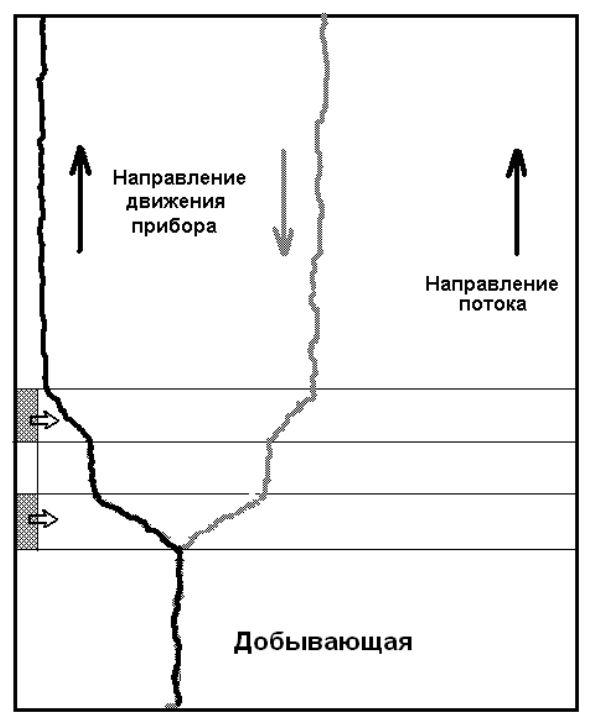
\includegraphics[width=.4\linewidth]{graph_2a}
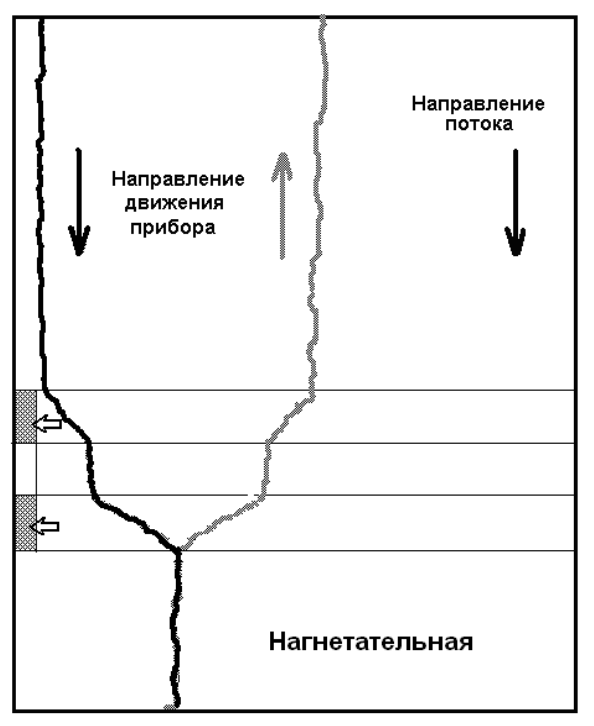
\includegraphics[width=.4\linewidth]{graph_2b}
\caption{
Типовая диаграмма механического
расходомера в интервале
пласта, регистрируемая в
добывающей и нагнетательной скважине
на спуске и подъеме
}
\label{fig:graph_2}
\end{figure}

\begin{figure}[!h]
\centering
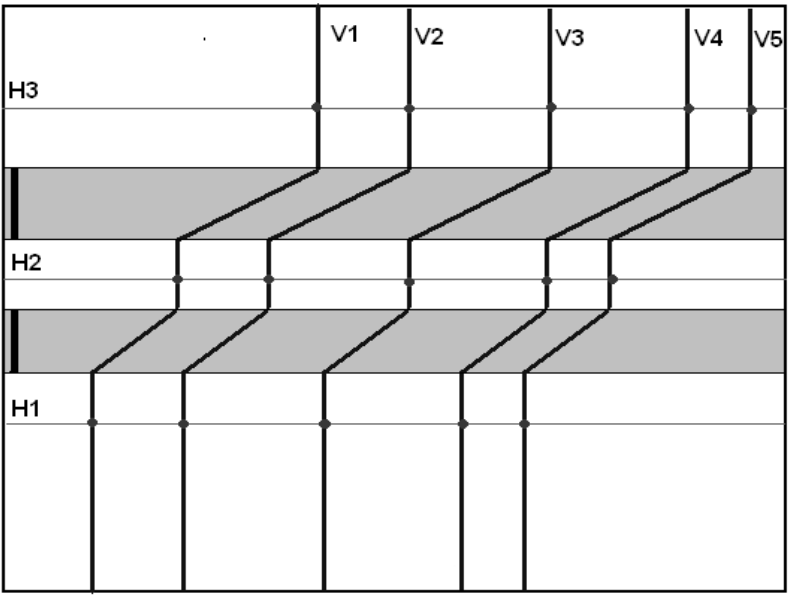
\includegraphics[width=.49\linewidth]{graph_3a}
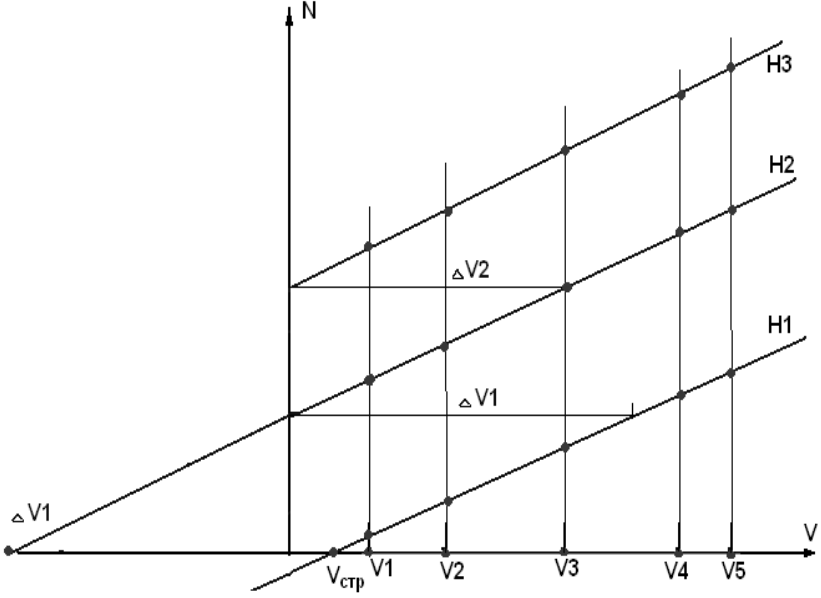
\includegraphics[width=.49\linewidth]{graph_3b}
\caption{
Типовые диаграммы механической расходометрии на
скоростях выполненные в интервалах притока и алгоритм обработки
замеров на скоростях. Замеры выполнены навстречу потоку. $\Delta Q = \frac 1 4 \pi D^2 \Delta V$,
где $Q$ --- расход жидкости, $D$ --- внутренний диаметр скважины,
$\Delta V$ --- приращение скорости жидкости;
}
\label{fig:graph_3}
\end{figure}

\clearpage
